\section{Governing Equations of MPM}
%Flow of information to communicate to the reader
The full set of governing equations for the membrane compaction problem discussed in the previous section is summarized as,

\begin{align}
\rho J-\rho_0=0
\label{Eq:mce}
\end{align}

\begin{align}
\rho \dot{\mathbf{v}} = \rho \mathbf{b} + \nabla . \sigma
\end{align}

The equation ofconservation of mass is not solved explicitly. Instead it is used to calculate the updated density field in the computations through Eq.~\ref{Eq:mce}. Like in many finite-element formulations, the method of weighted residuals is used to reduce the residual (error) to zero in an average sense. By taking the virtual displacement $\delta u_j \in \Re_0, \Re_0=\left\{\delta u_j\left|\delta u_j \in C^0, \delta u_j\right|_{\Gamma_u}=0\right\}$ as the test function, one obtains the weak form of the governing equations and the traction boundary condition as,

\begin{align}
	\begin{array}{r}
\int_{\Omega} \delta u_i\left(\sigma_{i j, j}+\rho b_i-\rho \ddot{u}_i\right) \mathrm{d} V=0, \\
\int_{\Gamma_t} \delta u_i\left(\sigma_{i j} n_j-\bar{t}_i\right) \mathrm{d} V=0,
\end{array}
\end{align}

which upon simplification is shown below.

\begin{align}
\int_{\Omega} \rho \ddot{u}_i \delta u_i \mathrm{~d} V+\int_{\Omega} \rho \sigma_{i j}^s \delta u_{i, j} \mathrm{~d} V-\int_{\Omega} \rho b_i \delta u_i \mathrm{~d} V-\int_{\Gamma_t} \rho \bar{t}_i^s \delta u_i \mathrm{~d} A=0
\label{Eq:GovEqMPM}
\end{align}

In the standard formulation of MPM used in this study, the density field in the domain is approximated as,
\begin{align}
\rho(\boldsymbol{x})=\sum_{p=1}^{n_p} m_p \delta\left(\boldsymbol{x}-\boldsymbol{x}_p\right)
\label{Eq:rho_def}
\end{align}

In the above equation, ${n_p}$ is the number of material points. Substituting Eq.~\ref{Eq:rho_def} in Eq.~\ref{Eq:GovEqMPM} and invoking particle quadrature, one obtains the numerical governing equation of MPM.  

\begin{align}
\sum_{p=1}^{n_p} m_p \ddot{u}_{i p} \delta u_{i p}+\sum_{p=1}^{n_p} m_p \sigma_{i j p}^s \delta u_{i p, j}-\sum_{p=1}^{n_p} m_p b_{i p} \delta u_{i p}-\sum_{p=1}^{n_p} m_p \bar{t}_{i p}^s h^{-1} \delta u_{i p}=0
\label{Eq:NumEqMPM}
\end{align}
The subscipts $p$ and $i$ refer to the particle and spatial dimension respectively. The solution of the numerical governing equation above is carried out in four stages as briefly discussed in the following sub-sections.
\subsection{Particle to Grid Interpolation (P2G)}
In this step, the material points are assumed to be attached to the background grid as shown in Figure~\ref{Fig:MPM_Steps}(a). The background grid is then considered similar to a finite element grid and based on the shape function defined at the grid node $I$ the unknown quantities in Eq.~\ref{Eq:NumEqMPM} are calculated as,
\begin{align}
\begin{array}{r}
u_{i p}  =N_{I p} u_{i I} \\
u_{i p, j}  =N_{I p, j} u_{i I}\\
\delta u_{i p} =N_{I p} \delta u_{i I}
\end{array}
\label{Eq:shape}
\end{align} 
In the equations above, subscript $I$ is used to denote the grid node and $N_I$ indicate the shape function defined at node $I$. In this study, two shape functions namely, the linear-hat and cubic spline shape functions are considered.
Substituting equations Eq.~\ref{Eq:shape} in Eq.~\ref{Eq:NumEqMPM} and cancelling the common virtual displacement term $\delta u_{i I}$, one obtains,
\begin{align}
m_{I J} \dot{u}_{i J}=f_{i I}^{\mathrm{int}}+f_{i I}^{\mathrm{ext}}, \quad x_I \notin \Gamma_u
\end{align} 

where $m_{I J}$ is the elements of the mass matrix defined as,
\begin{align}
m_{I J}=\sum_{p=1}^{n_p} m_p N_{I p} N_{J p}\\
\end{align}
 
and $f_{i I}^{\mathrm{int}}$ and $f_{i I}^{\mathrm{ext}}$ are the internal and external forces respectively and given by,
\begin{align}
f_{i I}^{\mathrm{int}}=-\sum_{p=1}^{n_p} N_{I p, j} \sigma_{i j p} \frac{m_p}{\rho_p} \\
f_{i I}^{\mathrm{ext}}=\sum_{p=1}^{n_p} m_p N_{I p} b_{i p}+\sum_{p=1}^{n_p} N_{I p} \bar{t}_{i p} h^{-1} \frac{m_p}{\rho_p}
\end{align}
Hence, this step of the MPM solution procedure involves 'projecting' properties from  material points to grid nodes and is shown schematically in Figure~\ref{Fig:MPM_Steps}(a).

\subsection{Temporal integration at grid nodes}
Once the grid nodal properties are calculated in the P2G operation, the updated velocity at grid nodes are calculated. In this study, a simple forward Euler time integration procedure is used. Since this procedure in its original form involves costly inversion of the mass matrix $m_{I J}$, the following mass-lumping approximation is made,

\begin{align}
m_I=\sum_{J=1}^{n_g} m_{I J}=\sum_{p=1}^{n_p} m_p N_{I p}
\end{align}

The velocity components at the nodes are then calculated as,
\begin{align}
\mathbf{v_{I}}^{t+\Delta t}=\mathbf{v_{I}}^{t}+\frac{1}{m_I} \left(\mathbf{f_{i I}}^{\mathrm{int}}+\mathbf{f_{i I}}^{\mathrm{ext}}\right)
\end{align}

where $\Delta t$ is the time step used in time integration and is calculated from the following equation,
\begin{align}
\Delta t= CFL \min \left(\frac{h_x}{c_x}, \frac{h_y}{c_y}, \frac{h_z}{c_z}\right)
\end{align}

Here, $c_()$ and $h_()$ refer to characteristic velocity and grid sizes in different directions respectively.

\subsection{Grid to Particle (G2P) Interpolation}
Once the updated velocities at grid nodes are obtained, the velocities and their gradients at the material points are obtained in this step as, 

\begin{align}
\mathbf{v}_p^{t+\Delta t}=\alpha_{P-F}\left(\mathbf{v}_p^t+\sum_I N_I \left[{\mathbf{v}}_I^{t+\Delta t}-\mathbf{v}_I^t\right]\right)+(1-\alpha_{P-F}) \sum_I N_I {\mathbf{v}}_I^{t+\Delta t}\\
\nabla \mathbf{v}_p^{t+\Delta t}=\sum_I^{ng} \nabla N_I \mathbf{v}_I^{t+\Delta t}
\end{align}

The term $\alpha_{P-F}$ used in the material point velocity update step above determines the level of blending between Particle-in-Cell (PIC) and Fluid Implicit Particle Method (FLIP) like updates.
The velocity gradient thus calculated at the material point is used to compute the stress tensor through the user-provided constitutive relation. 

\subsection{Material point position update and grid reset}
At this step, the updated velocity at the material point is already obtained and is used to update the material point position as,
\begin{align}
\mathbf{x}_{p}^{t+\Delta t}=\mathbf{x}_{p}^{t} +\Delta t \: \mathbf{v}_p^{t+\Delta t}
\end{align}

The background grid in MPM is used only as a scratch pad to calculate gradients and for time integration and hence is often reset or regenerated at the end of each MPM step.


\begin{figure}[h]
\subfloat[Particle to grid (P2G) operation]{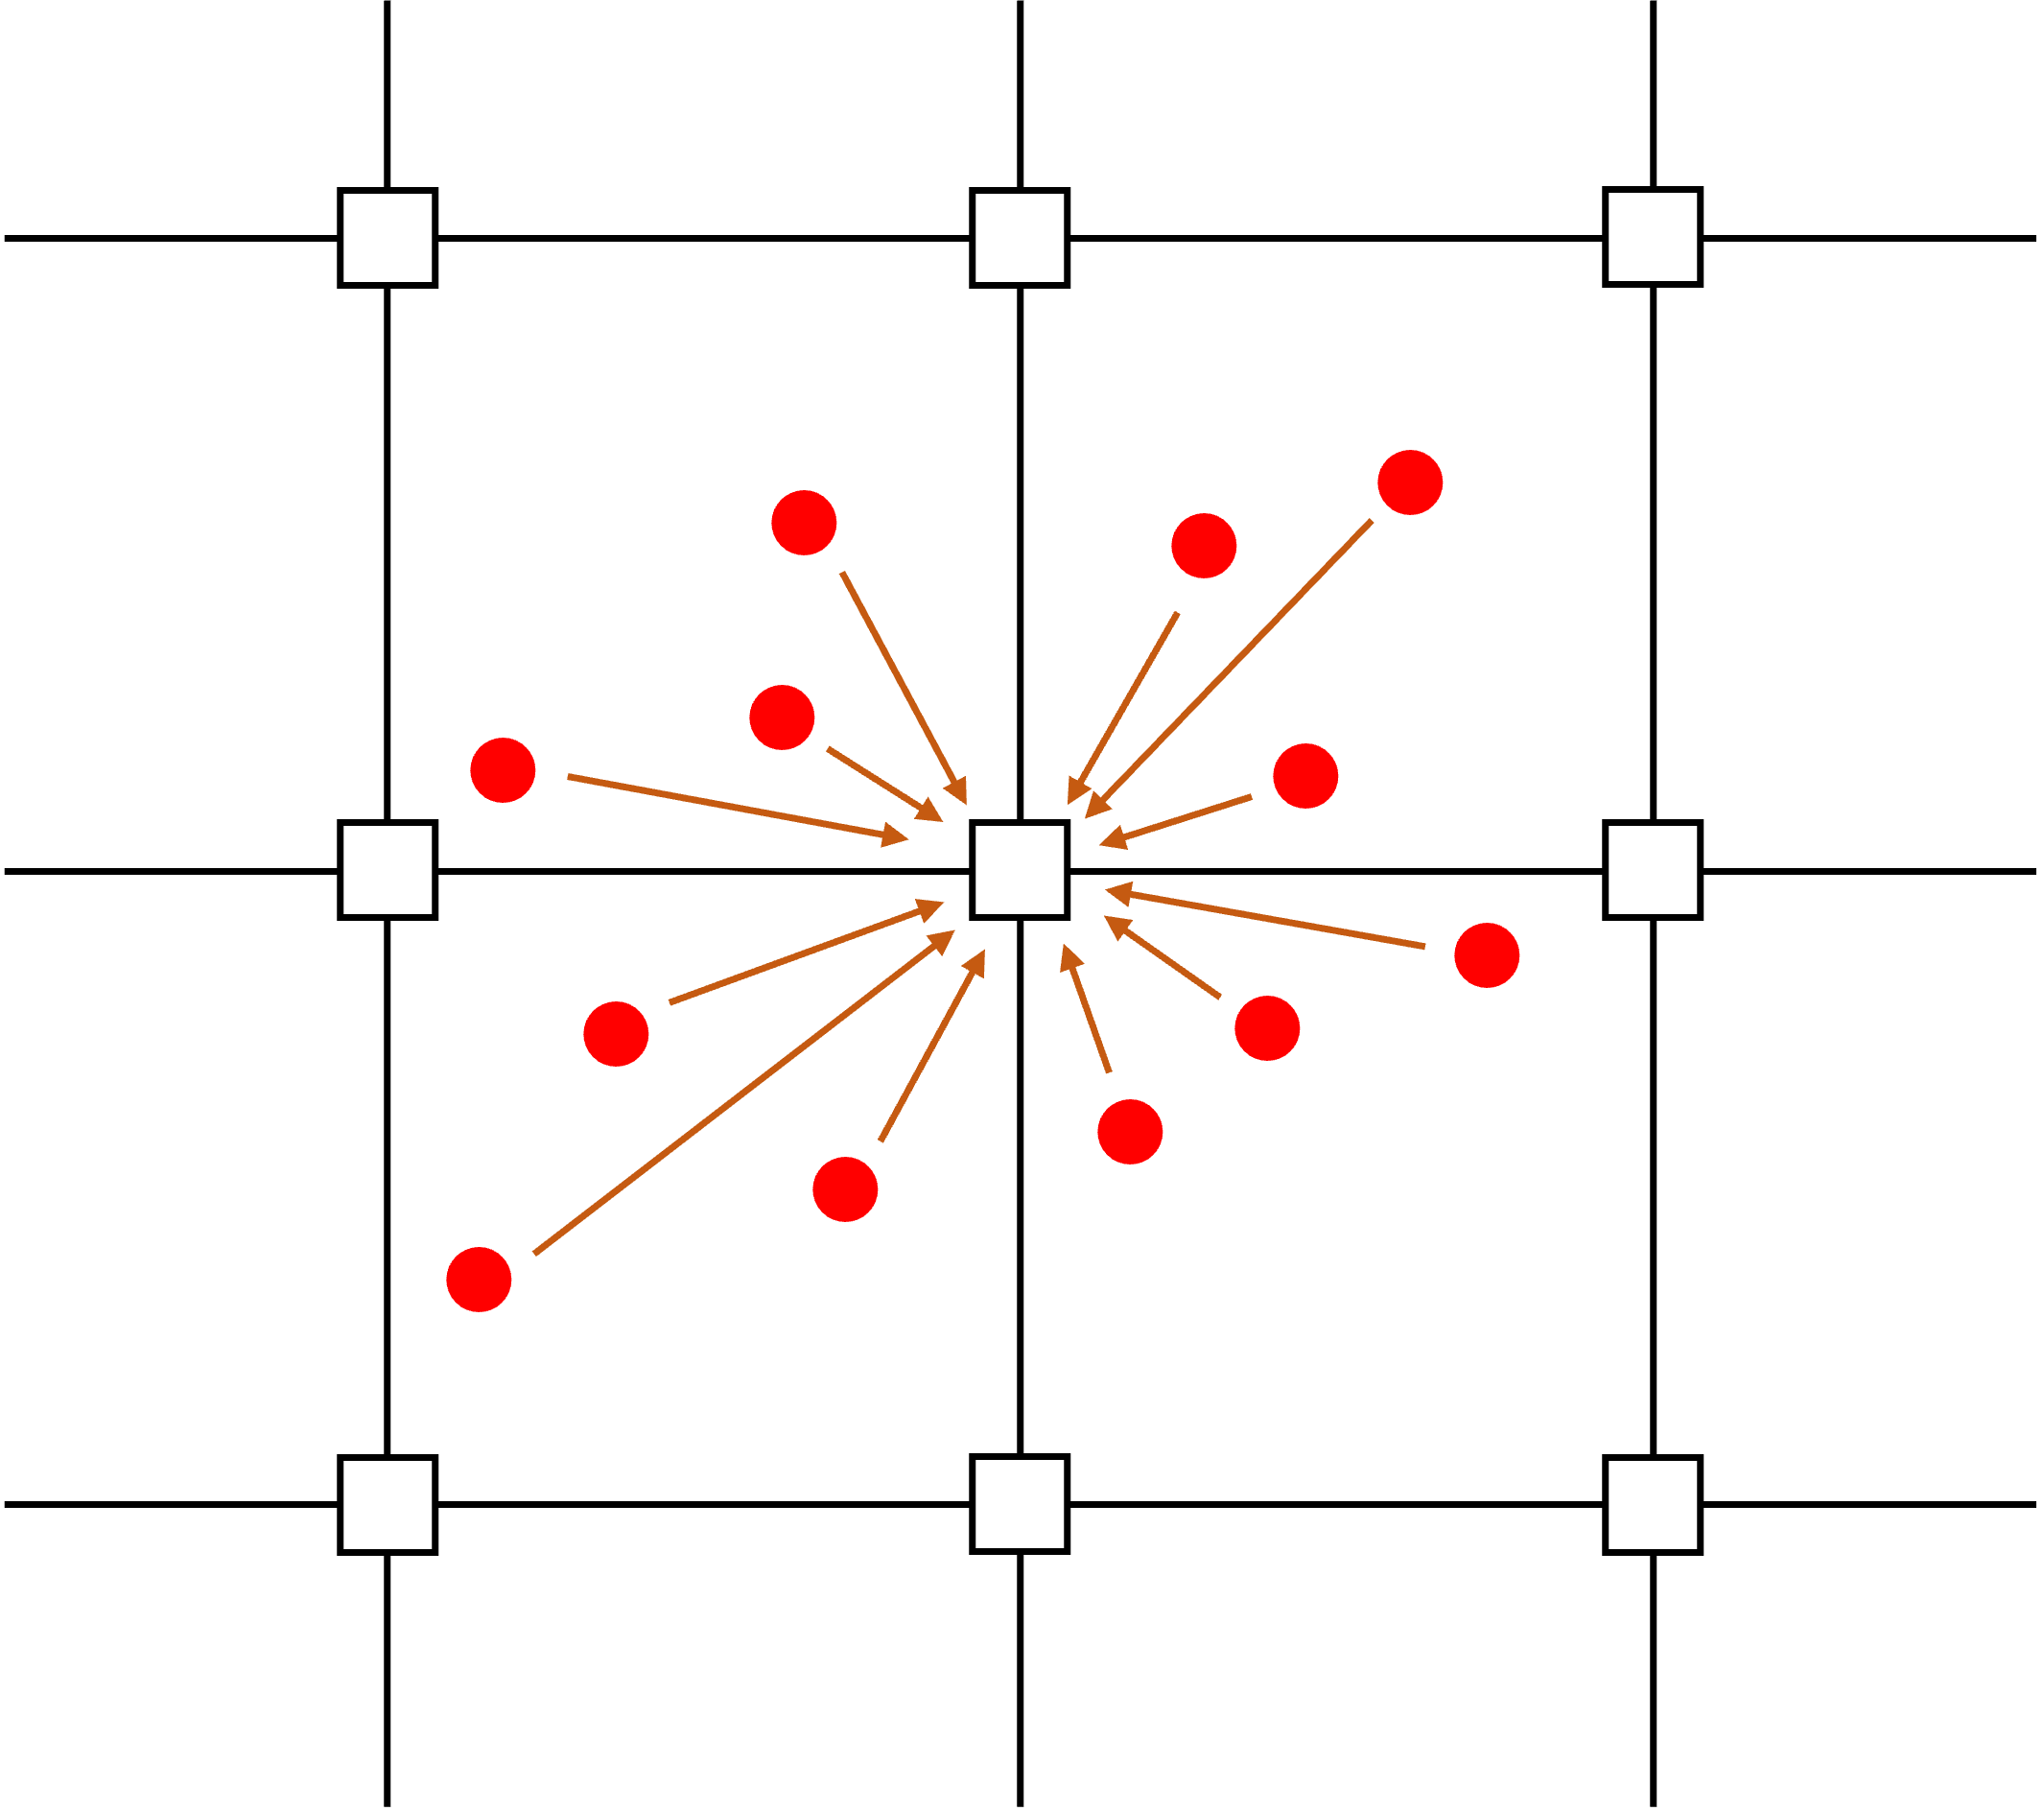
\includegraphics[width=0.4\textwidth]{./PICS/MPM_Step1.png}}
\subfloat[Nodal velocity update]{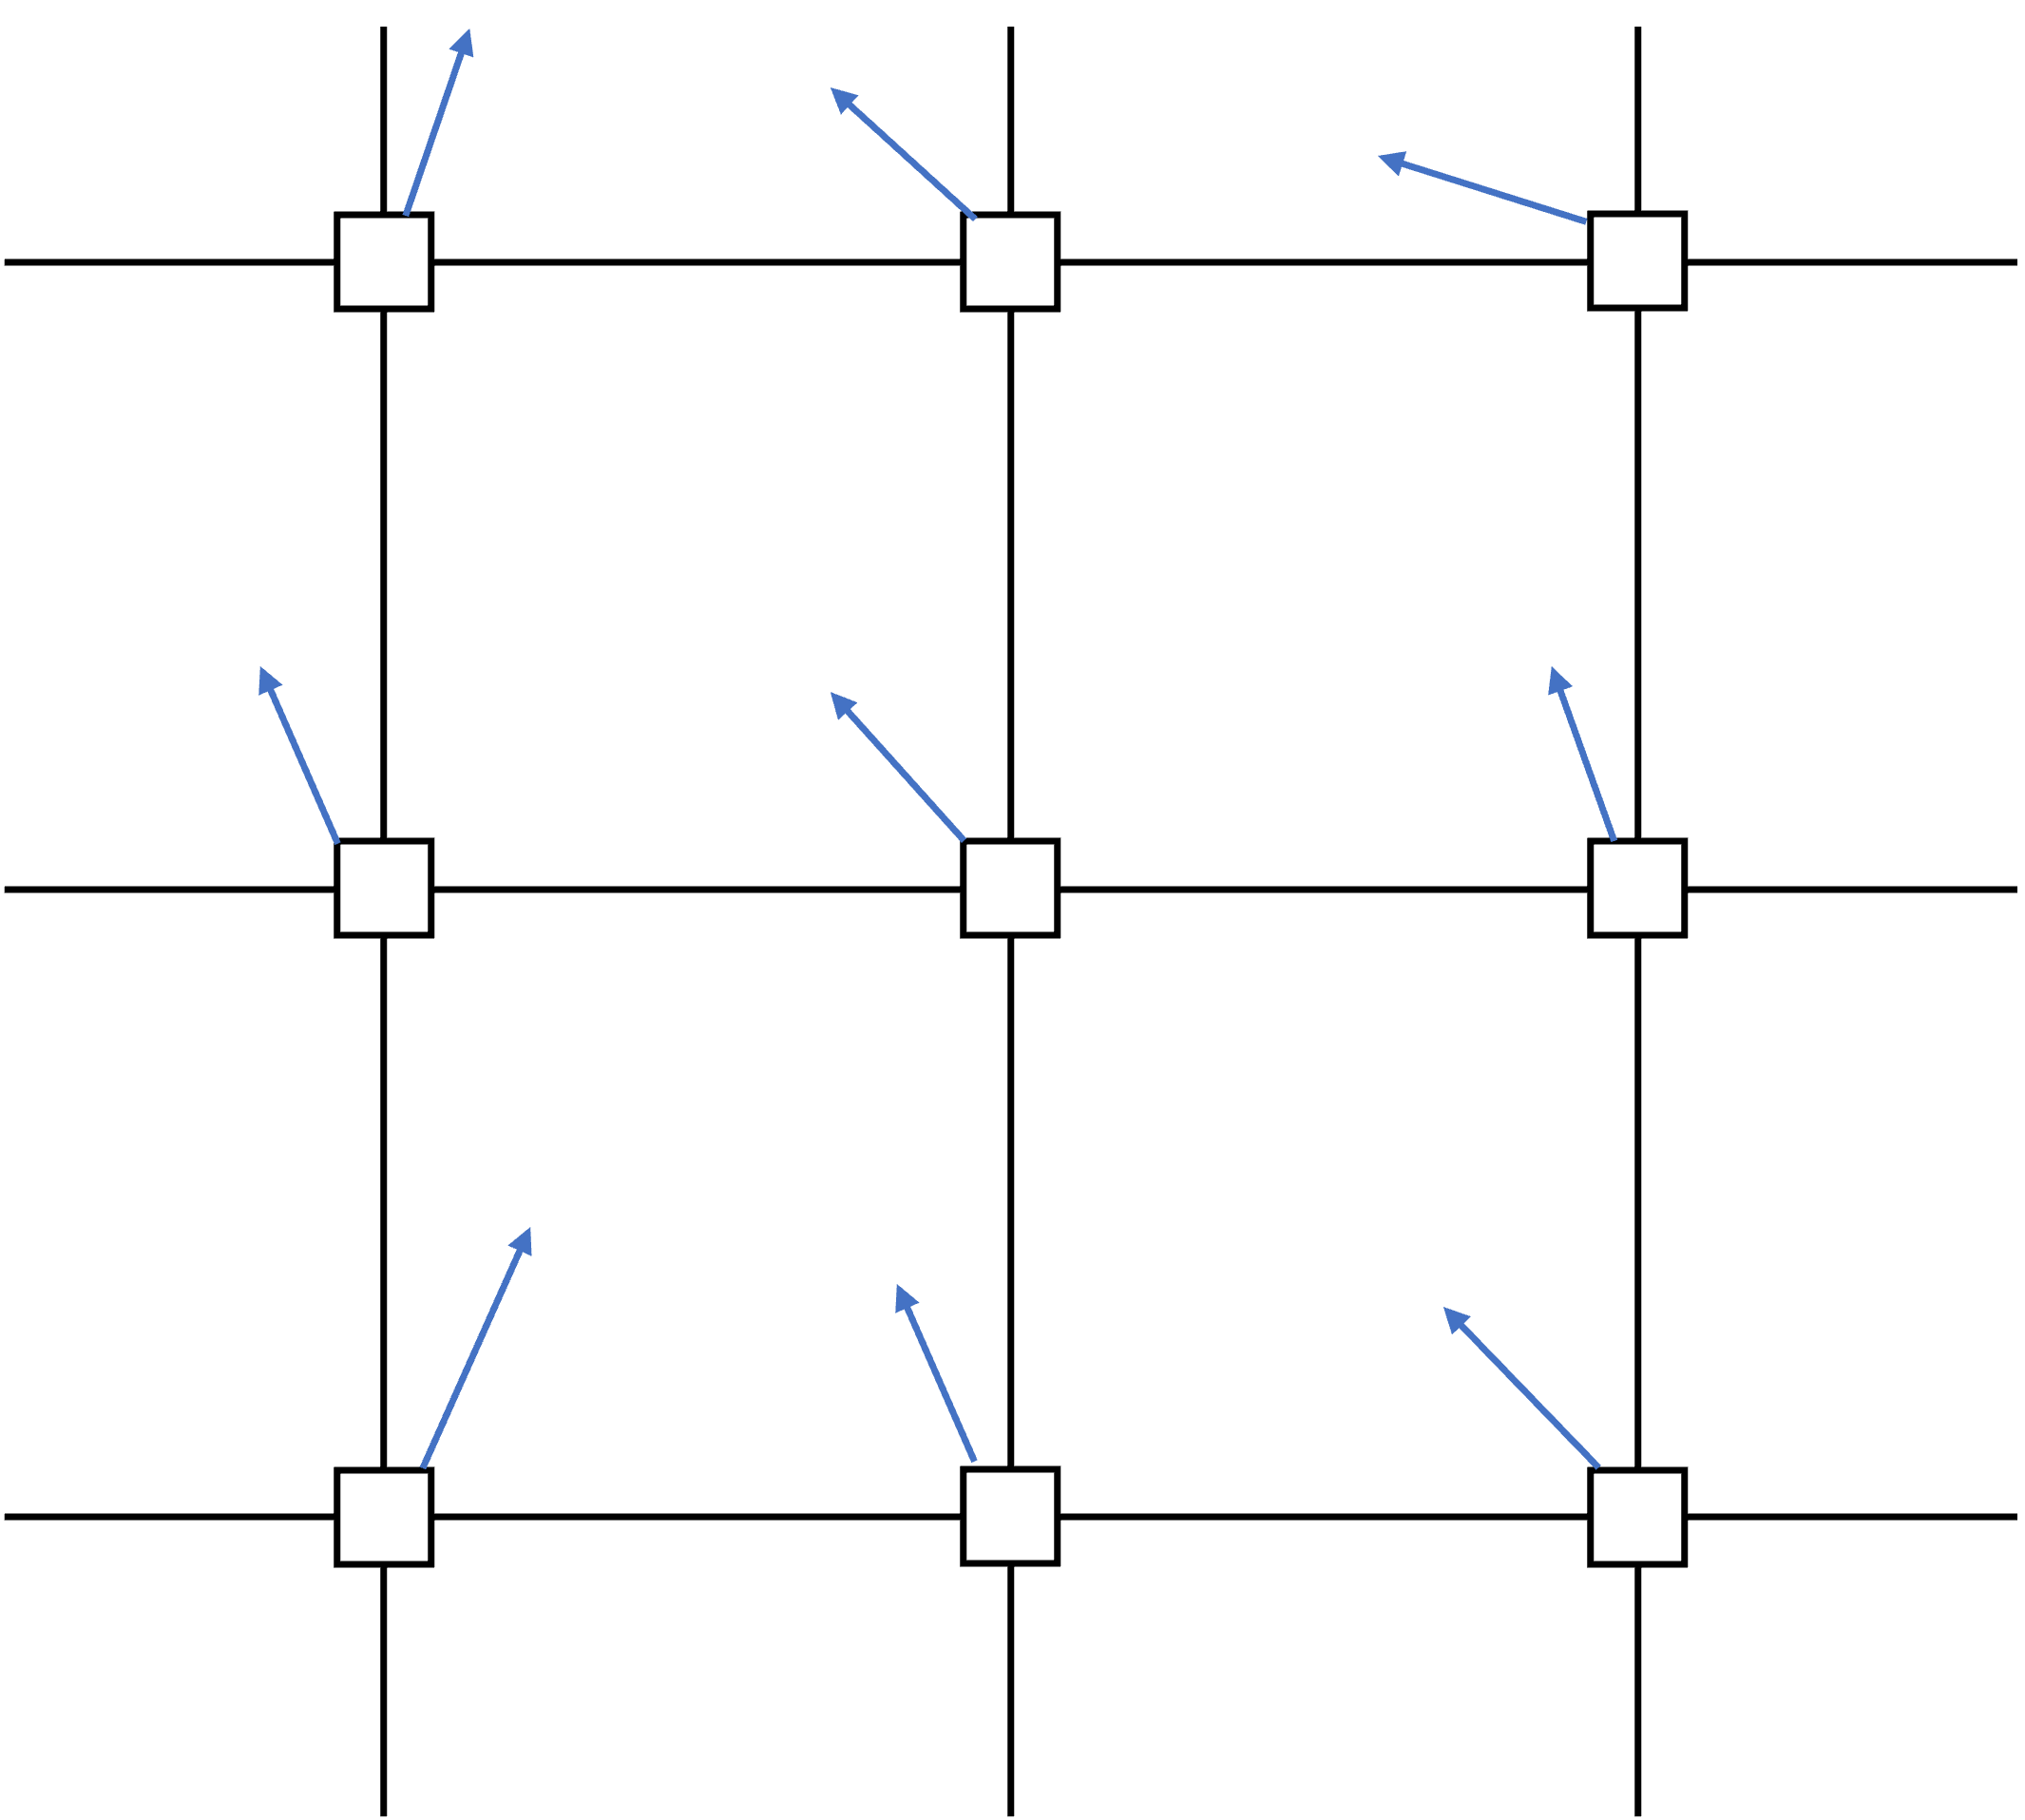
\includegraphics[width=0.4\textwidth]{./PICS/MPM_Step2.png}}\\
\subfloat[Grid to particle (G2P) operation]{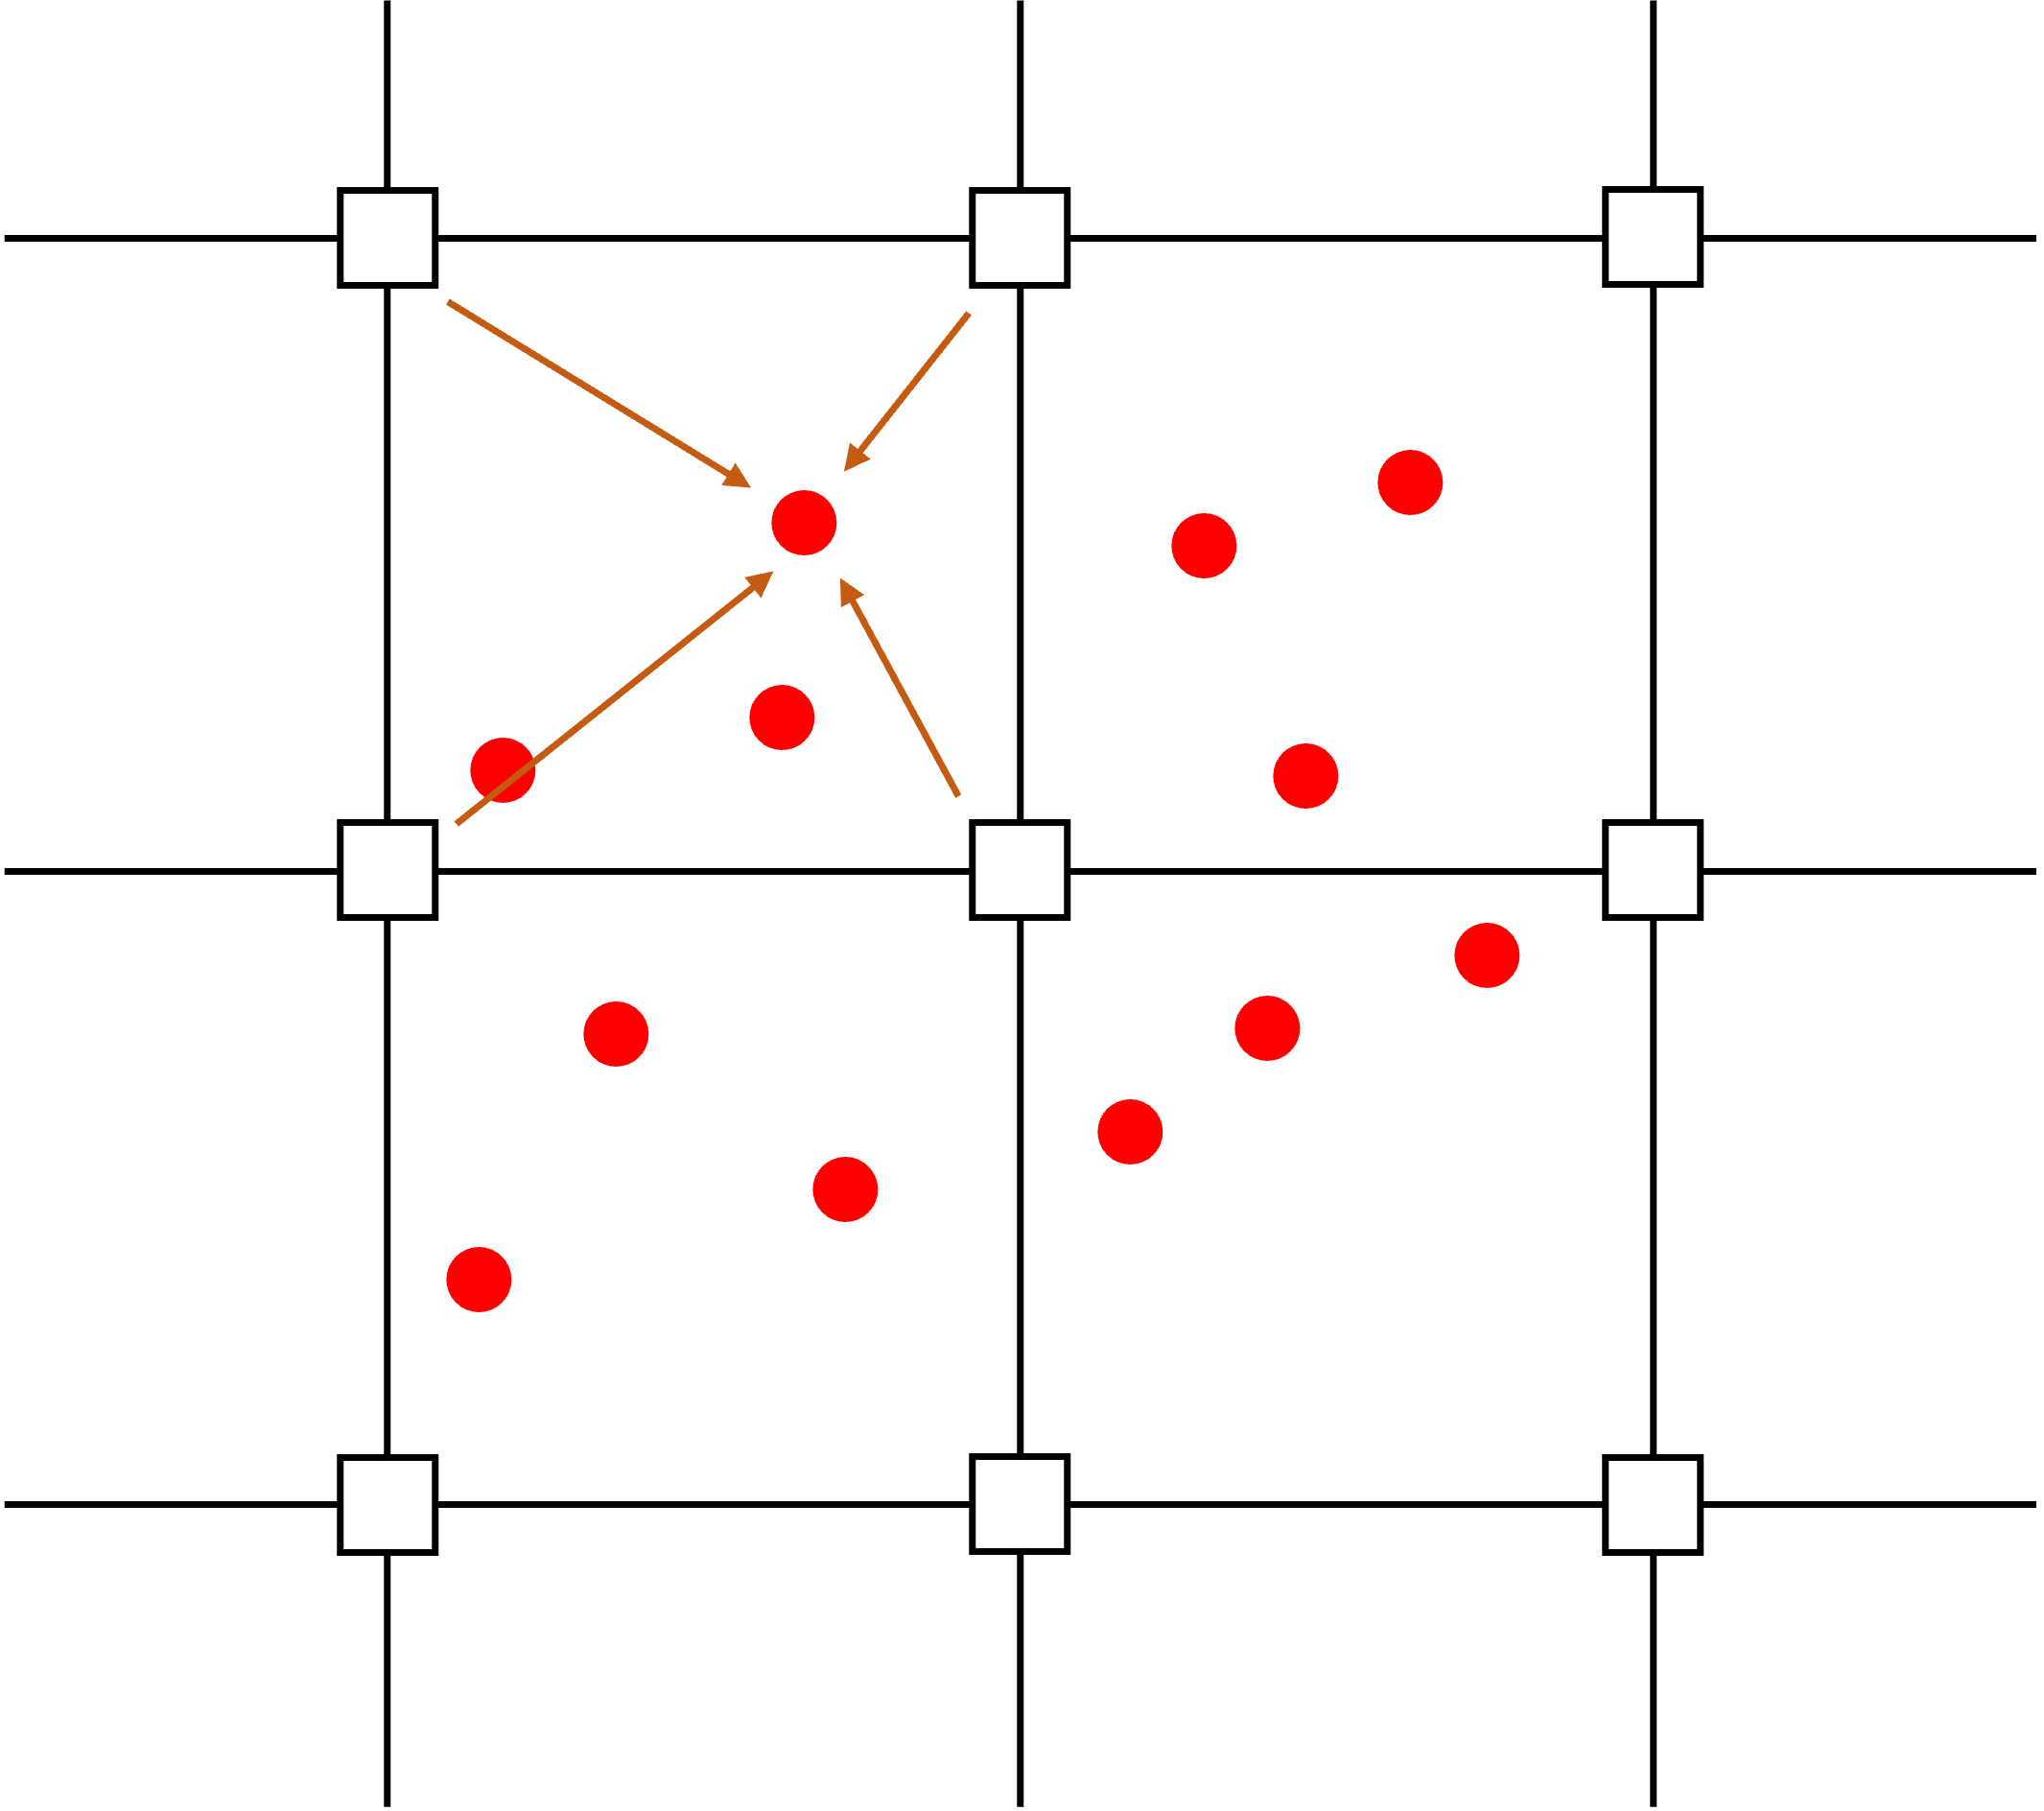
\includegraphics[width=0.4\textwidth]{./PICS/MPM_Step4.png}}
\subfloat[Particle position update]{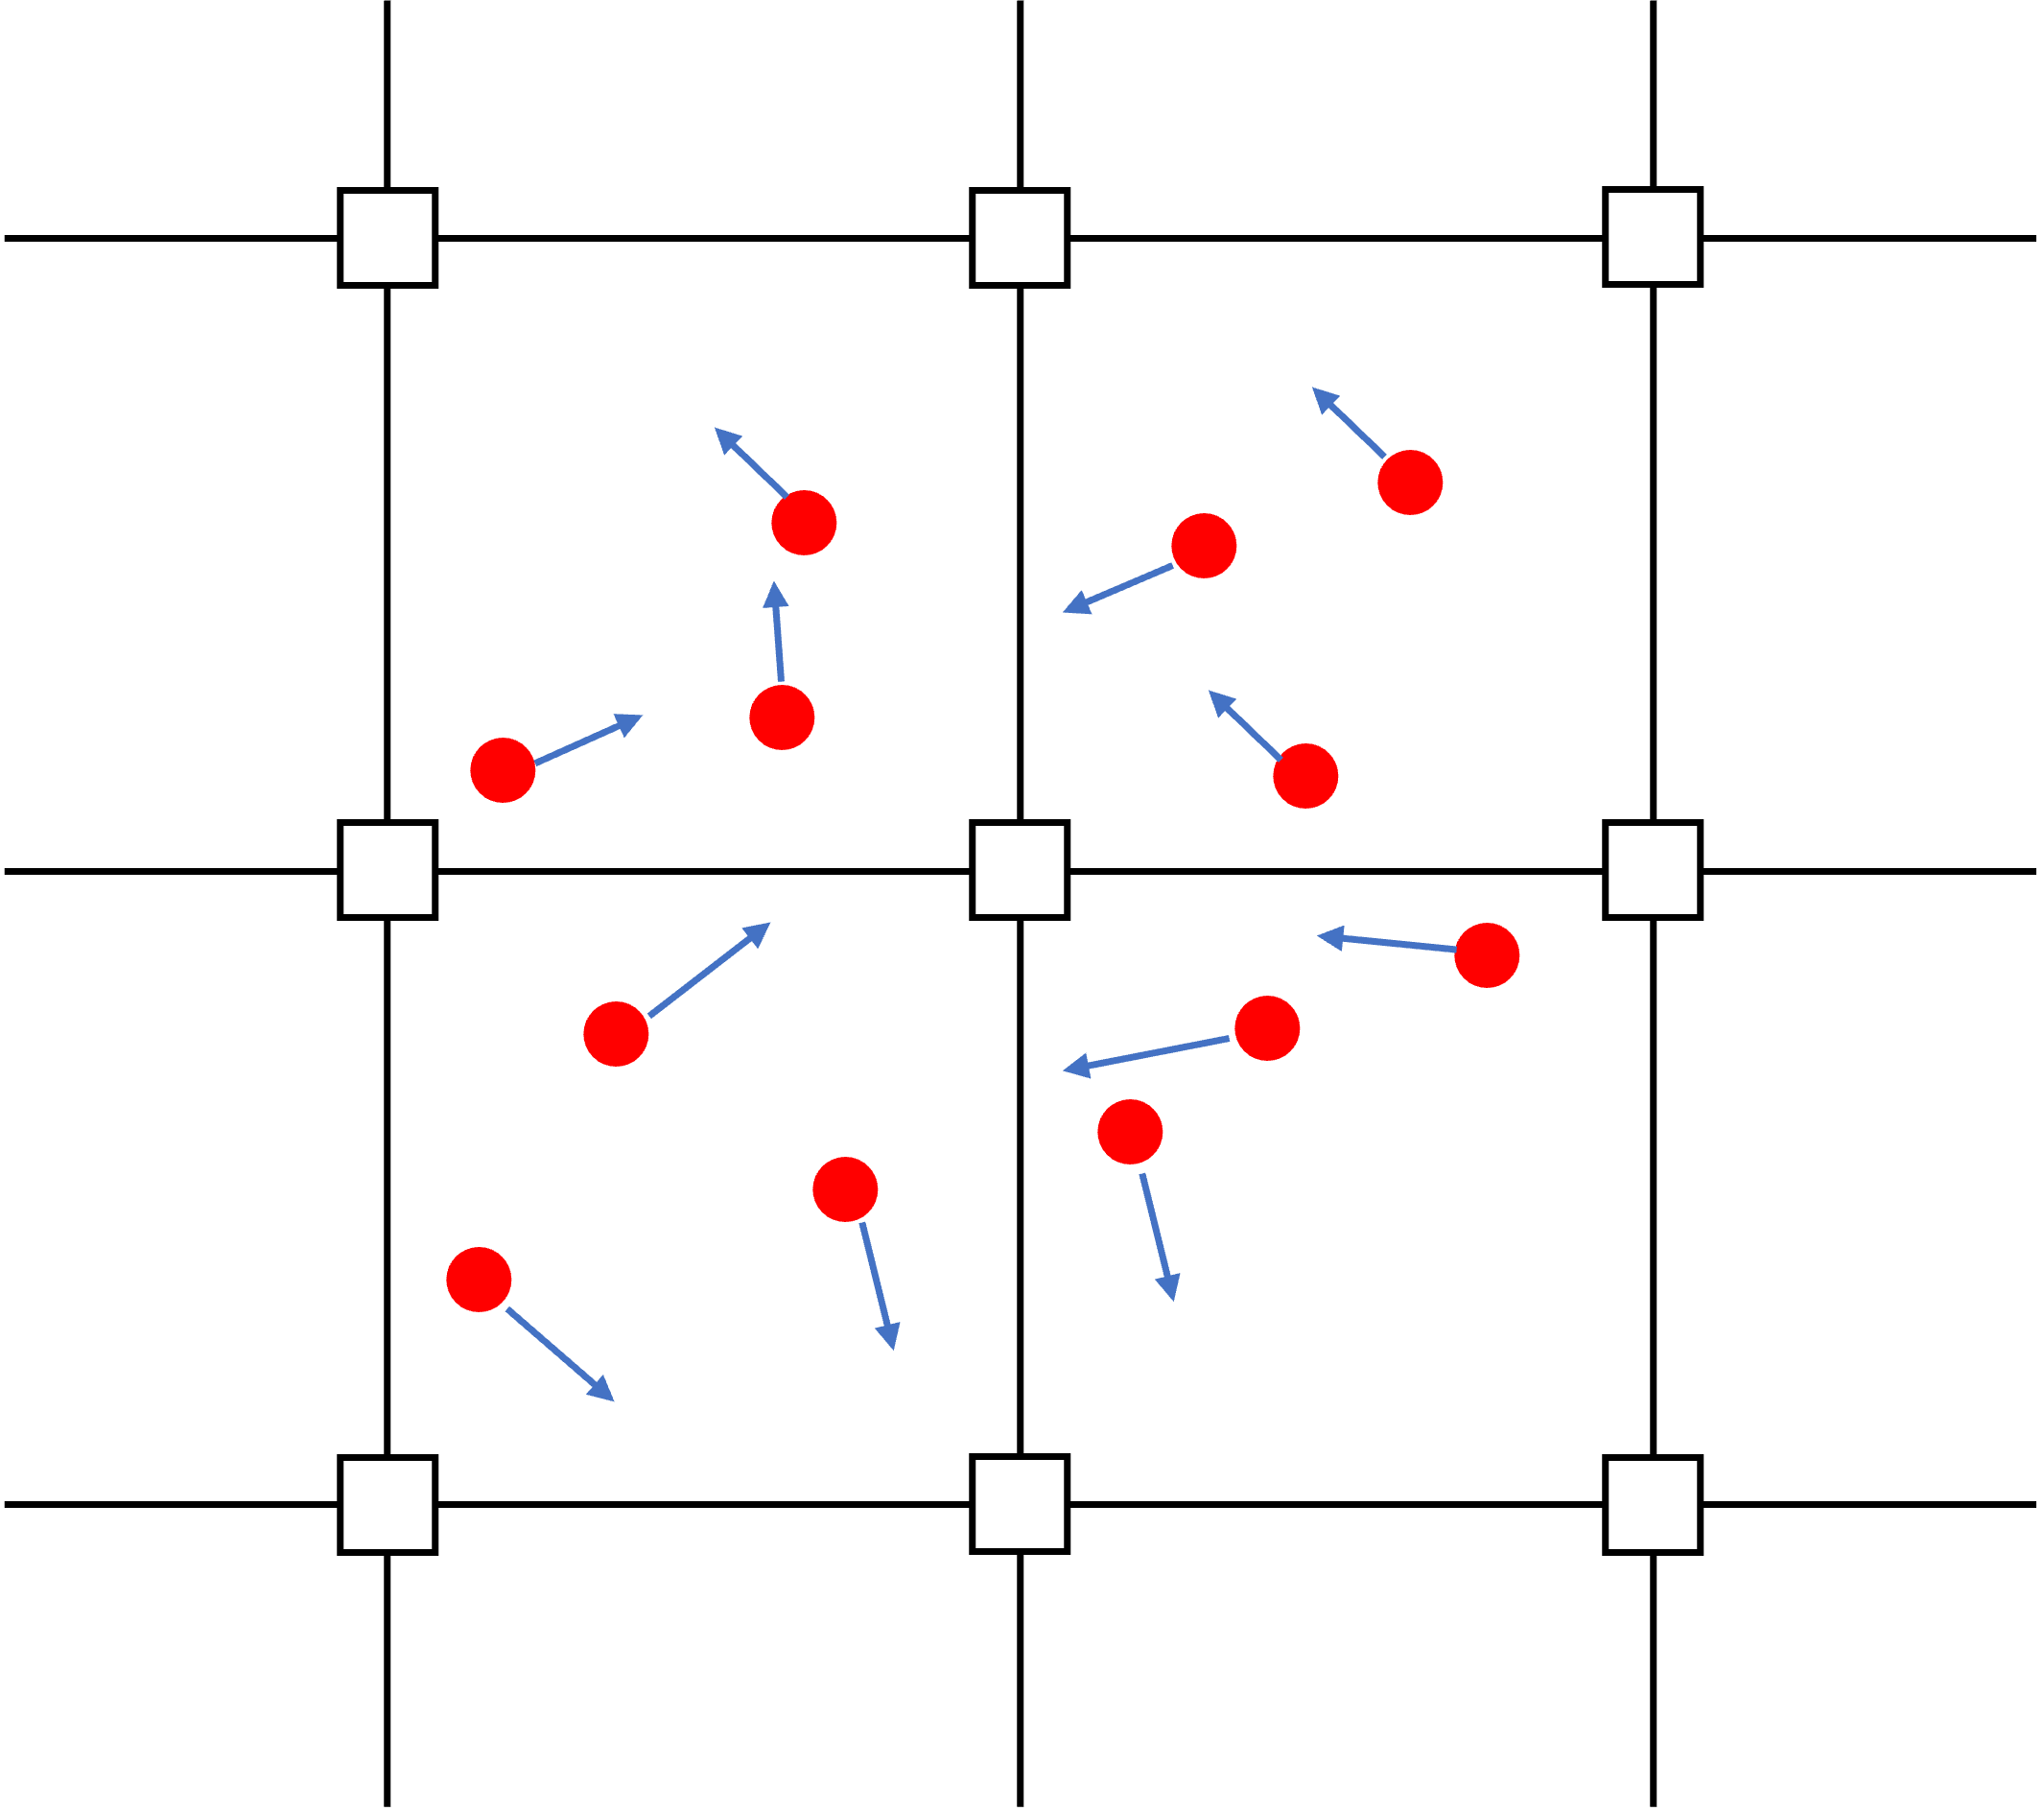
\includegraphics[width=0.4\textwidth]{./PICS/MPM_Step3.png}}
\caption{Various stages in MPM computations. The square symbols and associated lines indicate grid nodes and cell edges respectively. The background grid in most MPM codes is cartesian due to ease of grid generation. The red circles indicate material points}
\label{Fig:MPM_Steps}
\end{figure}